\documentclass{beamer}
\usepackage[utf8]{inputenc}
\usepackage[french]{babel}
\usepackage{xmpmulti}
\usepackage{amsmath}
\usepackage{amsfonts}
\usepackage{amssymb}
\usepackage{wasysym}
\usetheme{Warsaw}
\usecolortheme{beaver}
\setbeamertemplate{navigation symbols}{}
\usepackage{tikz}
\usetikzlibrary{calc}

\definecolor{pbblue}{HTML}{0A75A8}% color for the progress bar and the circle

\makeatletter
\def\progressbar@progressbar{} % the progress bar
\newcount\progressbar@tmpcounta% auxiliary counter
\newcount\progressbar@tmpcountb% auxiliary counter
\newdimen\progressbar@pbht %progressbar height
\newdimen\progressbar@pbwd %progressbar width
\newdimen\progressbar@rcircle % radius for the circle
\newdimen\progressbar@tmpdim % auxiliary dimension

\progressbar@pbwd=\linewidth
\progressbar@pbht=1pt
\progressbar@rcircle=2.5pt

% the progress bar
\def\progressbar@progressbar{%

    \progressbar@tmpcounta=\insertframenumber
    \progressbar@tmpcountb=\inserttotalframenumber
    \progressbar@tmpdim=\progressbar@pbwd
    \multiply\progressbar@tmpdim by \progressbar@tmpcounta
    \divide\progressbar@tmpdim by \progressbar@tmpcountb

  \begin{tikzpicture}
    \draw[pbblue!30,line width=\progressbar@pbht]
      (0pt, 0pt) -- ++ (\progressbar@pbwd,0pt);

    \filldraw[pbblue!30] %
      (\the\dimexpr\progressbar@tmpdim-\progressbar@rcircle\relax, .5\progressbar@pbht) circle (\progressbar@rcircle);

    \node[draw=pbblue!30,text width=3.5em,align=center,inner sep=1pt,
      text=pbblue!70,anchor=east] at (0,0) {\insertframenumber/\inserttotalframenumber};
  \end{tikzpicture}%
}

\setbeamertemplate{footline}
{%
  \begin{beamercolorbox}[wd=\paperwidth,ht=4ex,center,dp=1ex]{white}%
    \progressbar@progressbar%
  \end{beamercolorbox}%
}


\setbeamertemplate{headline}{}
\newcommand{\argmin}{\operatornamewithlimits{argmin}} 

\title[P300 BCI without training]{OpenplacOS : Automate your DIY system}
\author[A. Barachant, V. Lagorsse]{Vincent Lagorsse, Alexandre Barachant}\institute{}
\date{RMLL 2013}
\makeatother

\AtBeginSection[]{
{
\setbeamertemplate{footline}{} 
   \begin{frame}{Plan}
   %%% affiche en début de chaque section, les noms de sections et
   %%% noms de sous-sections de la section en cours.
   \tableofcontents[currentsection,hideothersubsections]
   \end{frame} 
   }
\addtocounter{framenumber}{-1}
}
	

\begin{document}

{
\setbeamertemplate{footline}{} 
\begin{frame}
  \titlepage
\end{frame}
}
\addtocounter{framenumber}{-1}

\section{Introduction}

\begin{frame}{Introduction}
\begin{block}{OpenplacOS}
Automation for DIY systems
\end{block}
\end{frame}

\begin{frame}{Examples}
\begin{columns}
\begin{column}[l]{0.5\textwidth}
\begin{figure}
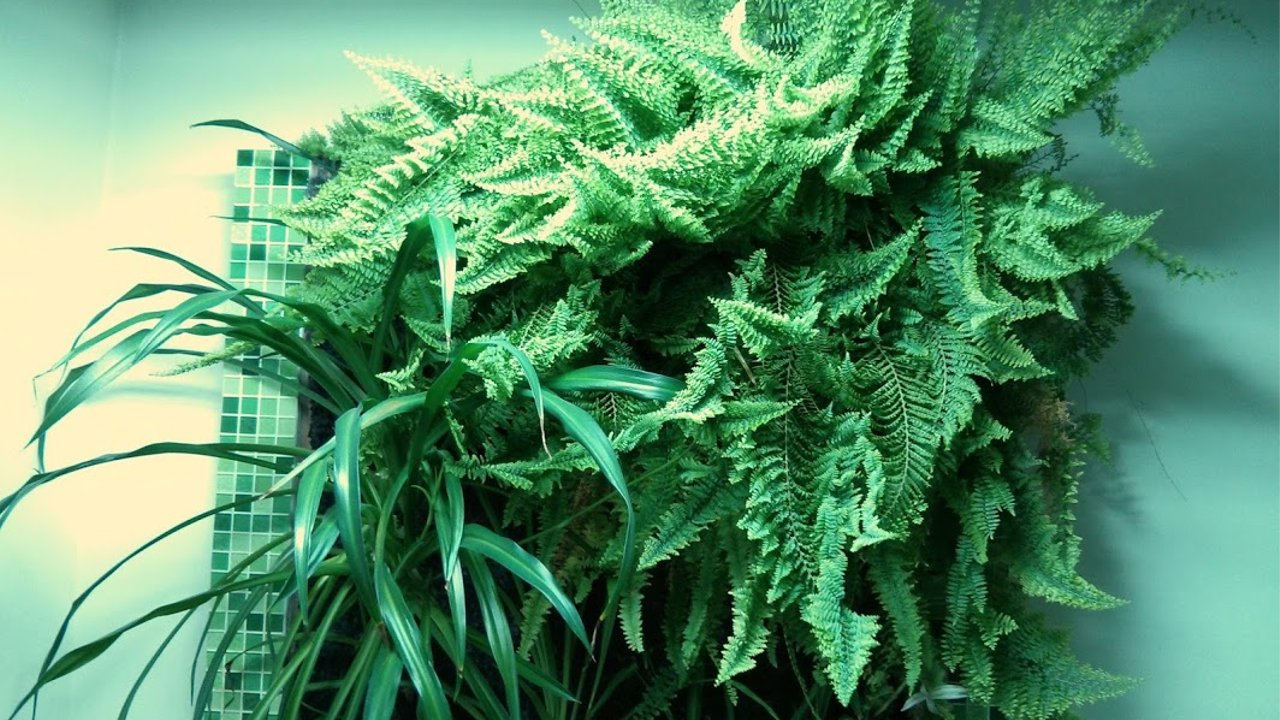
\includegraphics[width=\columnwidth]{./figures/mur.jpg}
\end{figure}
\vfill
\textbf{Aquariums, Indoor garden :}
\begin{itemize}
\item Lights
\item Pumps
\item Watering
\item Nutriement, pH
\item Temperature, $\mathrm{CO}_2$
\end{itemize}
\end{column}
\begin{column}[r]{0.5\textwidth}
\textbf{DIY Brewery :}
\begin{itemize}
\item Temperature
\item Process control
\end{itemize}
\vfill
\begin{figure}
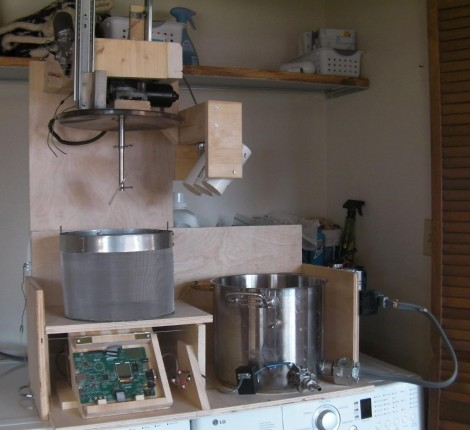
\includegraphics[width=0.8\columnwidth]{./figures/brewery.jpg}
\end{figure}
\end{column}
\end{columns}
\end{frame}

\begin{frame}{Hardware Solutions}
\begin{columns}
\begin{column}[l]{0.5\textwidth}
\textbf{Commercial products :}
\begin{itemize}
\item Expensive
\item Closed
\item No Fun !
\end{itemize}
\end{column}
\begin{column}[r]{0.5\textwidth}
\begin{figure}
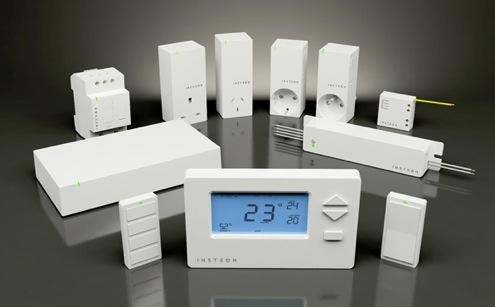
\includegraphics[width=\columnwidth]{./figures/Home-Automation-Products.jpg}
\end{figure}
\end{column}
\end{columns}

\begin{columns}
\begin{column}[l]{0.5\textwidth}
\textbf{DIY / Open Hardware :}
\begin{itemize}
\item Flexible
\item Time Consuming
\item Require electronic and programming skills
\end{itemize}
\end{column}
\begin{column}[r]{0.5\textwidth}
\begin{figure}
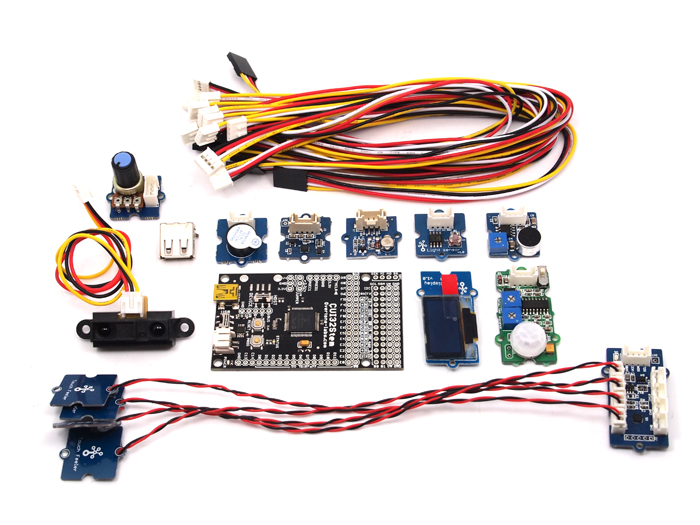
\includegraphics[width=\columnwidth]{./figures/kit.jpg}
\end{figure}
\end{column}
\end{columns}
\end{frame}

\begin{frame}{Software Solutions}
\begin{columns}
\begin{column}[l]{0.5\textwidth}
\textbf{Home Automation software :}
\begin{itemize}
\item Not adapted
\end{itemize}
\end{column}
\begin{column}[r]{0.5\textwidth}
\begin{figure}
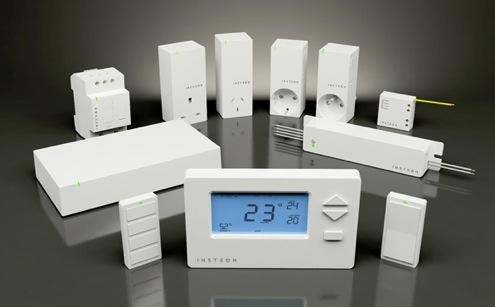
\includegraphics[width=\columnwidth]{./figures/Home-Automation-Products.jpg}
\end{figure}
\end{column}
\end{columns}

\begin{columns}
\begin{column}[l]{0.5\textwidth}
\textbf{DIY / Embed software  :}
\begin{itemize}
\item Hardware specific
\end{itemize}
\end{column}
\begin{column}[r]{0.5\textwidth}
\begin{figure}
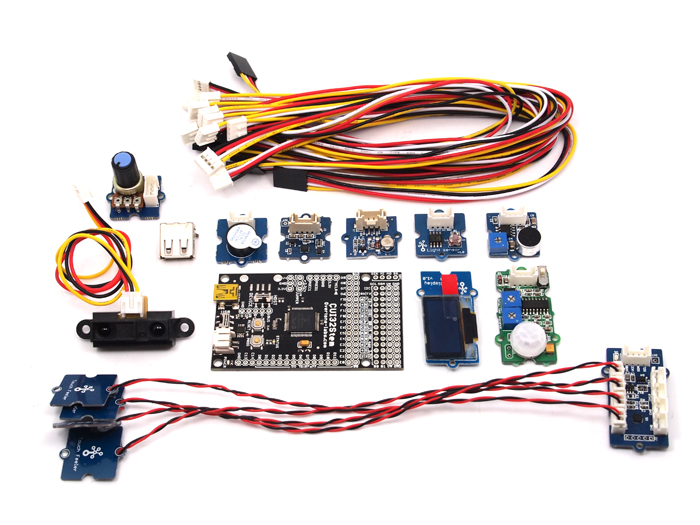
\includegraphics[width=\columnwidth]{./figures/kit.jpg}
\end{figure}
\end{column}
\end{columns}
\end{frame}

\begin{frame}{OpenplacOS}
\begin{block}{OpenplacOS is designed to be :}
\begin{itemize}
\item Flexible
\item Modular
\item Hardware independant
\item Easy to configure \& to use
\end{itemize}
\end{block}
\end{frame}

\section{Workflow}

\section{Software Architecture}

\section{Demo}

\section{Conclusion}

\end{document}